\documentclass[10pt,fleqn]{article} % Default font size and left-justified equations
\usepackage[%
    pdftitle={Dynamique : Inertie équivalente},
    pdfauthor={Xavier Pessoles}]{hyperref}
    
\input{style/new_style}
\input{style/macros_SII}

\usepackage{multicol}
\usepackage{style/schemabloc}
\fichetrue
%\fichefalse

\proftrue
%\proffalse

\tdtrue
%\tdfalse

%\courstrue
\coursfalse

\def\discipline{Sciences \\Industrielles de \\ l'Ingénieur}
\def\xxtete{Sciences Industrielles de l'Ingénieur}

\def\classe{PT -- PT$\star$}
\def\xxnumpartie{Partie n}
\def\xxpartie{Méthode de résolution permettant la détermination les actions mécaniques dans les liaisons ou les lois de déplacement en dynamique\\
Analyse, Modélisation, Résolution}

\def\xxnumchapitre{Chapitre n}
\def\xxchapitre{Titre Chapitre}

\def\xxtitreexo{Exercices d'application}
\def\xxsourceexo{\hspace{.2cm}}


\def\xxposongletx{2}
\def\xxposonglettext{1.45}
\def\xxposonglety{20}
\def\xxonglet{Part. ** -- Ch. **}

\def\xxactivite{Applications}
\def\xxauteur{\textsl{Xavier Pessoles}}

\def\xxcompetences{%
\textsl{%
\textbf{Savoirs et compétences :}\\
\noindent \textbf{Résoudre :} à partir des modèles retenus :
\begin{itemize}[label=\ding{112},font=\color{ocre}] 
\item ***
\item ***
\end{itemize}
\begin{itemize}[label=\ding{112},font=\color{ocre}] 
\item ***
\end{itemize}
%
%\noindent \textit{Mod2 -- C4.1 :} Représentation par schéma bloc.
}}

\def\xxfigures{
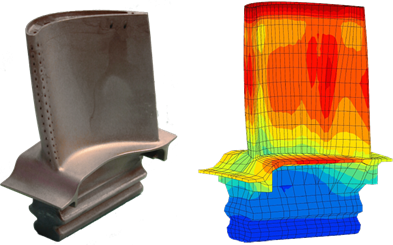
\includegraphics[width=.8\textwidth]{images/rdm}
}%figues de la page de garde

\def\xxpied{%
Partie * -- ** -- Analyse, Modélisation, Résolution \\
Ch. * : ** -- \xxactivite%
}


\setcounter{secnumdepth}{5}
%---------------------------------------------------------------------------


\begin{document}
%\chapterimage{png/Fond_Cin}
\input{style/new_pagegarde}
\vspace{10cm}
\pagestyle{fancy}
\thispagestyle{plain}


\def\columnseprulecolor{\color{ocre}}
\setlength{\columnseprule}{0.4pt} 

%\begin{multicols}{2}

\section*{Exercice 1 -- Calcul de l'inertie équivalente d'un train épicycloïdal}
\setcounter{subparagraph}{0}

On considère le train épicycloïdal suivant à trois satellites. Chacune des pièces est axisymétrique. On donne leurs matrices d'inertie :
$$
\overline{\overline{I_A}}(1/0) = 
\begin{pmatrix} 
A_1 & 0 & 0 \\
0 & B_1 & 0 \\
0 & 0 & C_1 \\
\end{pmatrix}
\quad
\overline{\overline{I_B}}(2/0) = 
\begin{pmatrix} 
A_2 & 0 & 0 \\
0 & B_2 & 0 \\
0 & 0 & C_2 \\
\end{pmatrix}
$$

$$
\overline{\overline{I_A}}(3/0) = 
\begin{pmatrix} 
A_3 & 0 & 0 \\
0 & B_3 & 0 \\
0 & 0 & C_3 \\
\end{pmatrix}
$$

\begin{center}
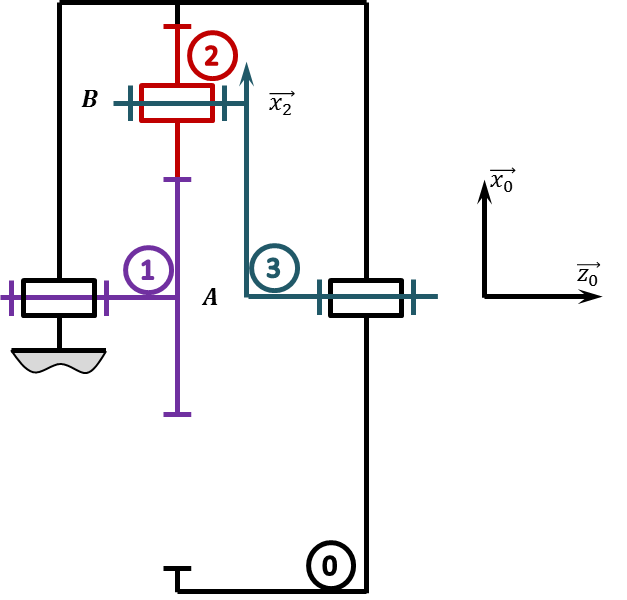
\includegraphics[width=.45\textwidth]{images/train_01}
\end{center}

On montre que : $\mu = \dfrac{\omega(2/0)}{\omega(1/0)}=-\dfrac{r_1}{2r_2}$ .

\subparagraph{}
\textit{Déterminer le rapport de réduction du train épicycloïdal.}
\ifprof
\begin{corrige}
\begin{methode}
\begin{enumerate}
\item Écrire le rapport de réduction recherché.
\item Refaire le schéma en fixant le porte satellite et en libérant le bâti. Le porte satellite devient donc le bâti et le train peut être considéra comme un train simple.
\item Déterminer le rapport de réduction du train simple (les taux de rotation seront donc exprimés en fonction du porte-satellite) en fonction du nombre de dents des roues dentées.
\item Introduire les fréquences de rotation exprimées au point 1.
\item Exprimer le rapport de réduction cherché en fonction du  nombre de dents des solides. 
\end{enumerate}
\end{methode}


\begin{minipage}[c]{.6\linewidth}
On recherche $k=\dfrac{\omega(3/0)}{\omega(1/0)}$. 

On bloque le porte satellite \textbf{3} et on libère la couronne \textbf{0}. 

On peut donc exprimer $ \dfrac{\omega(0/3)}{\omega(1/3)} = (-1)^1\dfrac{Z_1\cdot Z_2}{Z_2\cdot Z_0} = -\dfrac{Z_1}{Z_0}$.

En décomposant le taux de rotation, on introduit $\omega(1/0)$ et $\omega(0/3)$ :
$ \dfrac{\omega(0/3)}{\omega(1/3)} =  \dfrac{\omega(0/3)}{\omega(1/0)+\omega(0/3)} = -\dfrac{Z_1}{Z_0} 
\Leftrightarrow \dfrac{-\omega(3/0)}{\omega(1/0)-\omega(3/0)}  =-\dfrac{Z_1}{Z_0}  \Leftrightarrow {Z_0} \omega(3/0)  =Z_1 \left( \omega(1/0)-\omega(3/0)\right) 
\Leftrightarrow  \omega(3/0) \left(Z_0 + Z_1\right) =Z_1 \omega(1/0) 
\Leftrightarrow \dfrac{\omega(3/0)}{\omega(1/0)} = \dfrac{Z_1}{Z_1+Z_0}$.

Au final, $k = \dfrac{\omega(3/0)}{\omega(1/0)} = \dfrac{Z_1}{Z_1+Z_0}$.
\end{minipage}\hfill
\begin{minipage}[c]{.35\linewidth}
\begin{center}
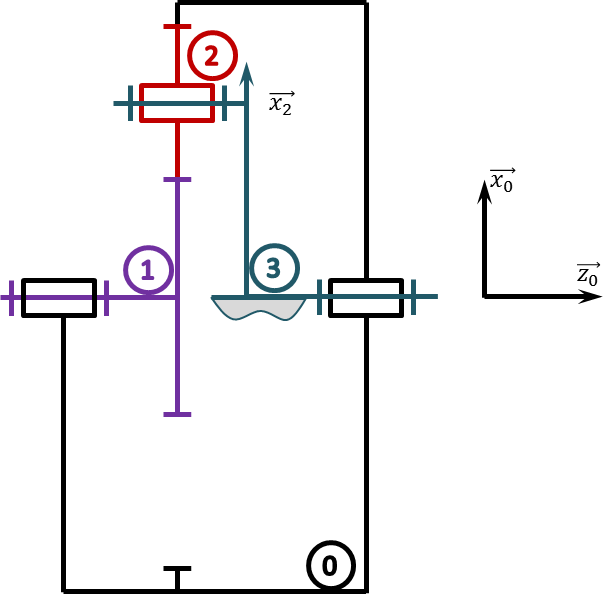
\includegraphics[width=\textwidth]{images/train_02}
\end{center}

\end{minipage}
\end{corrige}
\else
\fi

\subparagraph{}
\textit{Déterminer l'énergie cinétique de l'ensemble $E=\{1,2,3\}$ par rapport au référentiel de la pièce \textbf{0} supposé galiléen.}
\ifprof
\begin{corrige}
\begin{methode}
\begin{enumerate}
\item On calcule $T(1/0)$, 
\end{enumerate}
\end{methode}
\textbf{Calcul de l'énergie cinétique du planétaire : $T(1/0)$}

Par définition, 
$2T(1/0)=\left\{\mathcal{V}(1/0) \right\} \otimes \left\{\mathcal{C}(1/0) \right\} $
$A$ étant un point fixe dans \textbf{0}, on a : 
$$
\left\{\mathcal{V}(1/0) \right\} = \torseurl{\vecto{1}{0}=\omega(1/0)\vect{z_0}}{\vectv{A}{1}{0}=\vect{0}}{A}$$

$$
\left\{\mathcal{C}(1/0) \right\} 
= \torseurl{M_1\vectv{G}{1}{0}}{\vect{\sigma \left( A\in 1/0\right)}=\overline{\overline{I}}\left( A,0\right) \vecto{1}{0}=C_1\omega(1/0)\vect{z}}{A}
$$
On a donc : 
$$T(1/0)=\dfrac{1}{2} C_1 \omega(1/0)^2 $$

\end{corrige}

\begin{corrige}
\textbf{Calcul de l'énergie cinétique du porte-satellite : $T(3/0)$}

Par définition, 
$2T(2/0)=\left\{\mathcal{V}(2/0) \right\} \otimes \left\{\mathcal{C}(2/0) \right\} $; on a : 
$$
\left\{\mathcal{V}(3/0) \right\} = \torseurl{\vecto{3}{0}=\omega(3/0)\vect{z_0}}{\vectv{A}{3}{0}=\vect{0}}{A}
$$

$$
\left\{\mathcal{C}(3/0) \right\} 
= \torseurl{M_3\vectv{G}{3}{0}}{\vect{\sigma \left( A\in 3/0\right)}=\overline{\overline{I}}\left( A,3\right) \vecto{3}{0}=C_3\omega(3/0)\vect{z}}{A}
$$
On a donc : 
$$T(3/0)=\dfrac{1}{2} C_3 \omega(3/0)^2=\dfrac{1}{2} k^2 C_3 \omega(1/0)^2 $$


\end{corrige}

\begin{corrige}

\textbf{Calcul de l'énergie cinétique d'un seul satellite : $T(2/0)$}

Par définition, 
$2T(2/0)=\left\{\mathcal{V}(2/0) \right\} \otimes \left\{\mathcal{C}(2/0) \right\} $ et le centre d'inertie d'un porte satellite est au point $B$ on a donc : 
$$
\left\{\mathcal{V}(2/0) \right\} = \torseurl{\vecto{2}{0}=\omega(2/0)\vect{z_0}}{\vectv{B}{2}{0}}{B} 
$$

$$
\left\{\mathcal{C}(2/0) \right\} 
= \torseurl{M_2\vectv{G}{2}{0}}{\vect{\sigma \left( A\in 2/0\right)}=\overline{\overline{I}}\left( A,2\right) \vecto{2}{0}=C_2\omega(2/0)\vect{z}}{A}
$$

$\vectv{B}{2}{0}= \vectv{B}{2}{3} + \vectv{B}{3}{0} = \vect{0}  + \vectv{A}{3}{0} + \vect{BA} \wedge \vecto{3}{0} = -R_3 \vect{x_3} \wedge \omega(3/0) \vect{z_0}= -R_3\omega(3/0)\vect{y_3} $.

\begin{rem}
Le vecteur $\vect{AB}$ est porté par le porte satellite. Par ailleurs, les points $A$, $B$ ainsi que les points de contact dans les engrenages sont toujours suivant la direction du porte satellite. 
Enfin, $R_3=R_1+R_2$.
\end{rem}
D'où : 
$$
\left\{\mathcal{V}(2/0) \right\} = \torseurl{\vecto{2}{0}=\omega(2/0)\vect{z_0}}{\vectv{B}{2}{0}=-R_3\omega(3/0)\vect{y_3}}{B}  
$$

$$\left\{\mathcal{C}(2/0) \right\} 
= \torseurl{M_2\vectv{G}{2}{0}=-R_3\omega(3/0)\vect{y_3}}{\vect{\sigma \left( A\in 2/0\right)}=C_2\omega(2/0)\vect{z}}{A}
$$

On a donc : 
$$T(3/0)=\dfrac{1}{2} C_2 \omega(2/0)^2 + \dfrac{1}{2}M_2 R_3^2 \omega(3/0)^2 
= \dfrac{1}{2} C_2 \dfrac{r_1^2}{4r_2^2}\omega(1/0)^2 + \dfrac{1}{2}M_2 R_3^2 k^2 \omega(1/0)^2
=\dfrac{1}{2} C_2 \mu^2\omega(1/0)^2 + \dfrac{1}{2}M_2 R_3^2 \omega(3/0)^2 
 $$


\end{corrige}

\begin{corrige}

\textbf{Calcul de l'énergie cinétique de l'ensemble E: $T(E/0)$}

Sans oublier qu'il y a 3 satellites (...), on a donc :
$$T(E/0)=T(1/0)+T(2/0)+T(3/0) $$

$$T(E/0) = \dfrac{3}{2} C_2 \dfrac{r_1^2}{4r_2^2}\omega(1/0)^2 + \dfrac{3}{2}M_2 R_3^2 k^2 \omega(1/0)^2 + \dfrac{1}{2} C_1 \omega(1/0)^2 + \dfrac{1}{2} k^2 C_3 \omega(1/0)^2
$$
D'où 
$$T(E/0) = \dfrac{1}{2}\left( 3 C_2 \mu^2 + 3M_2 R_3^2 k^2 + C_1  +  k^2 C_3 \right)\omega(1/0)^2
$$

On note donc $J_{eq} = 3 C_2 \mu^2 + 3M_2 R_3^2 k^2 + C_1  +  k^2 C_3$ l'inertie équivalente du train épicycloïdal.
\end{corrige}

\begin{corrige}
\begin{methode}
\end{methode}
\end{corrige}

\begin{corrige}
\textbf{Calcul des puissances externes}

\textbf{Calcul des puissances dues aux actions de contact}

\textbf{Puissance dissipée dans la liaison pivot entre 1 et 0 : $\mathcal{P}_{0\rightarrow 1}$ :} 


On a : $\mathcal{P}_{0\rightarrow 1} = \torseurcin{V}{1}{0} \otimes \torseurstat{T}{1}{0}$
$$
\torseurcin{V}{1}{0} 
= \torseurl{\vecto{1}{0}=\omega(1/0)\vect{z_0}}{\vectv{A}{1}{0}=\vect{0}}{A}  
\quad 
\torseurstat{T}{1}{0}
= \torseurl{\vectf{1}{0}}{\vectm{A}{1}{0}=L_{01}\vect{x_0} + L_{01}\vect{y_0}}{A}  
$$

On a donc : $\mathcal{P}_{0\rightarrow 1} = 0$.

\begin{itemize}
\item \textbf{Puissance dissipée dans la liaison engrenage entre 2 et 0 : $\mathcal{P}_{0\rightarrow 2}=0$ } 
\item \textbf{Puissance dissipée dans la liaison pivot entre 3 et 0 : $\mathcal{P}_{0\rightarrow 3}=0$ } 
\item \textbf{Puissance fournie à l'arbre 1 : $\mathcal{P}_{\text{ext} \rightarrow 1} = C_e \omega(1/0)$} 
\item \textbf{Puissance transmise par l'arbre 3 : $\mathcal{P}_{\text{3} \rightarrow \text{ext}} = C_s \omega(3/0) = k C_s \omega(1/0) $} 
\item \textbf{Calcul des puissances dues aux actions à distance}

\item \textbf{Puissance due à la pesanteur sur la pièce 1}

\item \textbf{Puissance due à la pesanteur sur la pièce 3}

\item \textbf{Puissance due à la pesanteur sur la pièce 2}

\item \textbf{Calcul des puissances internes}

\item \textbf{Puissance dissipée dans la liaison engrenage entre 1 et 2 : $\mathcal{P}_{1\rightarrow 2} = 0$ (RSG)} 


\item \textbf{Puissance dissipée dans la liaison pivot entre 2 et 3 : $\mathcal{P}_{3\rightarrow 2} = 0$}

D'après le théorème de l'énergie puissance, on a : 
$$
\dfrac{\text{d}T\left(E/0\right)}{\text{d}t} = \left( C_e + kC_s\right)\omega(1/0)
\Leftrightarrow
J_{eq}\dot{\omega}(1/0) = \left( C_e + kC_s\right)
$$
\end{itemize} 
\end{corrige}

\else
\fi


%\end{multicols}
\end{document}



\subparagraph{}
\textit{}

\ifprof
\begin{corrige}
\end{corrige}
\else
\fi